% This file was created by matlab2tikz v0.0.7.
% Copyright (c) 2008--2010, Nico Schlömer <nico.schloemer@gmail.com>
% All rights reserved.
% 
% The latest updates can be retrieved from
%   http://www.mathworks.com/matlabcentral/fileexchange/22022-matlab2tikz
% where you can also make suggestions and rate matlab2tikz.
% 
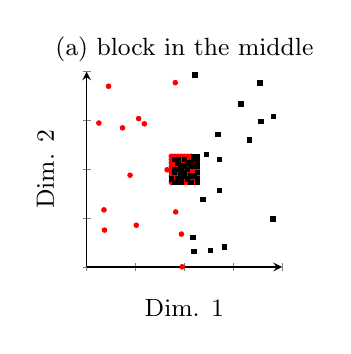
\begin{tikzpicture}

\begin{axis}[
footnotesize,
width= 1.6in,
height= 1.6in,
xmin=0, xmax=30,
ymin=0, ymax=30,
title={(a) block in the middle},
ytick={0,7.5,15,22.5,30},
xtick = {0,7.5,15,22.5,30},
xlabel = {Dim. 1},
ylabel = {Dim. 2},
xticklabels={,,,,},
yticklabels={,,,,},
axis on top,
axis y line = left,
axis x line = bottom
%legend entries={$optimal$,$rand$,$IVM$,$maxent$,$QBC2$,$QBC100$,$SVM$},
 %egend style={nodes=right}
]
\addplot [
color=red,
only marks,
mark=*,
mark options={scale = 0.4}
]
coordinates{ (13,13) (15,13) (15.5,13) (16.5,13) (13.5,13.5) (15,13.5) (16,13.5) (16.5,13.5) (13,14) (13.5,14) (14,14) (15.5,14) (17,14) (13,14.5) (14,14.5) (15.5,14.5) (16,14.5) (16.5,14.5) (13,15) (15,15) (16,15) (16.5,15) (17,15) (13,15.5) (13.5,15.5) (14,15.5) (15.5,15.5) (13,16) (13.5,16) (14.5,16) (15,16) (16.5,16) (13,16.5) (14.5,16.5) (15.5,16.5) (16,16.5) (13,17) (13.5,17) (14,17) (14.5,17) (15,17) (15.5,17) (16,17) (8.86203,21.9844) (1.87844,22.0987) (7.62888,6.41534) (5.50559,21.3585) (7.97933,22.783) (6.66413,14.0934) (2.66314,8.77752) (14.6582,0.0330902) (13.6696,8.46285) (2.74037,5.67331) (13.6087,28.3003) (12.3521,14.9273) (3.36577,27.7504) (14.5511,5.06006)
};
\label{plots:negatives}

\addplot [
color=black,
only marks,
mark=square*,
mark options={scale = 0.4}
]
coordinates{ (13.5,13) (14,13) (14.5,13) (16,13) (17,13) (13,13.5) (14,13.5) (14.5,13.5) (15.5,13.5) (17,13.5) (14.5,14) (15,14) (16,14) (16.5,14) (13.5,14.5) (14.5,14.5) (15,14.5) (17,14.5) (13.5,15) (14,15) (14.5,15) (15.5,15) (14.5,15.5) (15,15.5) (16,15.5) (16.5,15.5) (17,15.5) (14,16) (15.5,16) (16,16) (17,16) (13.5,16.5) (14,16.5) (15,16.5) (16.5,16.5) (17,16.5) (16.5,17) (17,17) (18.3773,17.3043) (24.9794,19.4896) (26.7589,22.3496) (17.8888,10.3495) (16.4577,2.38458) (20.4057,11.7607) (19.0268,2.51172) (20.4262,16.5161) (28.71,23.0737) (21.1403,3.08034) (16.3379,4.55224) (20.1516,20.3166) (23.7032,25.0623) (26.6266,28.273) (16.6152,29.476) (28.6434,7.37318)
};
\label{plots:positives}

\end{axis}
\end{tikzpicture}
